\documentclass{standalone}
\usepackage{tikz}
\usepackage{ctex,siunitx,ninecolors}
\usepackage{tkz-euclide}
\usepackage{amsmath}
\usetikzlibrary{patterns, calc}
\usetikzlibrary {decorations.pathmorphing, decorations.pathreplacing, decorations.shapes}
\newcommand\hand[2][0]{
    \begin{scope}[#2,rotate=#1]
    \fill[pink!10!orange!10,draw=black,very thin]
    ( 0.381,-0.532)..controls( 0.381,-0.532)and( 0.453,-0.637)..
    ( 0.528,-0.619)..controls( 0.569,-0.608)and( 0.617,-0.592)..
    ( 0.656,-0.559)..controls( 0.656,-0.559)and( 1.052,-0.743)..
    ( 1.265,-0.543)..controls( 1.265,-0.543)and( 1.394,-0.497)..
    ( 1.530,-0.522)..controls( 1.666,-0.548)and( 1.615, 0.055)..
    ( 1.615, 0.055)..controls( 1.615, 0.055)and( 1.419, 0.062)..
    ( 1.341, 0.100)..controls( 1.264, 0.138)and( 1.192, 0.195)..
    ( 1.000, 0.235)..controls( 0.809, 0.275)and( 0.544, 0.376)..
    ( 0.413, 0.370)..controls( 0.332, 0.366)and(-0.105, 0.228)..
    (-0.166, 0.109)..controls(-0.185, 0.072)and(-0.211,-0.006)..
    (-0.220,-0.076)..controls(-0.220,-0.076)and(-0.256,-0.256)..
    (-0.097,-0.285)..controls(-0.052,-0.297)and(-0.029,-0.260)..
    (-0.019,-0.245)..controls(-0.008,-0.229)and( 0.017,-0.315)..
    ( 0.040,-0.343)..controls( 0.063,-0.371)and( 0.097,-0.440)..
    ( 0.177,-0.440)..controls( 0.191,-0.441)and( 0.207,-0.442)..
    ( 0.223,-0.441)..controls( 0.223,-0.441)and( 0.282,-0.549)..
    ( 0.360,-0.536)..controls( 0.366,-0.535)and( 0.373,-0.534)..cycle;
  \draw[very thin]
  ( 0.752, 0.050)..controls( 0.752, 0.050)and( 0.479, 0.051)..
( 0.359, 0.091)..controls( 0.261, 0.123)and( 0.193, 0.129)..
( 0.071, 0.115)..controls(-0.052, 0.101)and(-0.178, 0.138)..
(-0.141,-0.040)..controls(-0.113,-0.173)and( 0.258,-0.180)..
( 0.337,-0.164)..controls( 0.366,-0.157)and( 0.510,-0.263)..( 0.640,-0.218)
(-0.016,-0.235)..controls( 0.002,-0.204)and( 0.011,-0.164)..( 0.007,-0.146)
(0.223,-0.441)..controls(0.312,-0.438)and(0.422,-0.404)..
(0.468,-0.291)..controls(0.476,-0.269)and(0.360,-0.166)..
(0.240,-0.242)..controls(0.226,-0.233)and(0.205,-0.224)..(0.219,-0.183)
(0.381,-0.532)..controls(0.473,-0.506)and(0.676,-0.401)..
(0.615,-0.331)..controls(0.586,-0.298)and(0.537,-0.260)..(0.472,-0.280)
(0.398,-0.262)..controls(0.420,-0.271)and(0.441,-0.285)..
(0.438,-0.301)..controls(0.435,-0.316)and(0.364,-0.387)..
(0.342,-0.382)..controls(0.344,-0.383)and(0.295,-0.348)..
(0.319,-0.309)..controls(0.343,-0.270)and(0.377,-0.252)..(0.398,-0.262)
(0.566,-0.236)..controls(0.566,-0.236)and(0.675,-0.413)..(1.099,-0.380)
(0.625, 0.066)..controls(0.625, 0.066)and(0.702, 0.114)..(0.801, 0.100)
(0.481, 0.073)..controls(0.481, 0.073)and(0.486, 0.167)..(0.509, 0.222)
(0.353, 0.096)..controls(0.353, 0.096)and(0.332, 0.155)..(0.338, 0.182)
(0.234,-0.017)..controls(0.234,-0.017)and(0.226, 0.063)..(0.233, 0.079)
(0.195,-0.010)..controls(0.195,-0.010)and(0.184, 0.064)..(0.196, 0.091)
(-0.130,-0.034)..controls(-0.130,-0.034)and( 0.023,-0.059)..
( 0.038,-0.028)..controls( 0.053, 0.003)and( 0.077, 0.079)..( 0.039, 0.109)
(0.228,-0.244)..controls(0.228,-0.244)and(0.166,-0.289)..(0.155,-0.319)
(0.318,-0.422)..controls(0.318,-0.422)and(0.266,-0.402)..(0.272,-0.370)
(0.492,-0.481)..controls(0.492,-0.481)and(0.459,-0.463)..(0.451,-0.445)
(0.541,-0.446)..controls(0.541,-0.446)and(0.489,-0.426)..
(0.508,-0.391)..controls(0.526,-0.356)and(0.565,-0.321)..(0.593,-0.328)
(0.656,-0.559)..controls(0.688,-0.532)and(0.715,-0.493)..
(0.728,-0.438)..controls(0.731,-0.403)and(0.666,-0.363)..(0.630,-0.386)
(0.687,-0.517)..controls(0.687,-0.517)and(0.613,-0.515)..
(0.631,-0.476)..controls(0.649,-0.438)and(0.666,-0.395)..(0.703,-0.399)
(0.636,-0.566)..controls(0.636,-0.566)and(0.602,-0.557)..(0.587,-0.522)
(1.329,-0.381)..controls(1.329,-0.381)and(1.481,-0.291)..(1.489,-0.356);
  \end{scope}
}
\begin{document}
\small
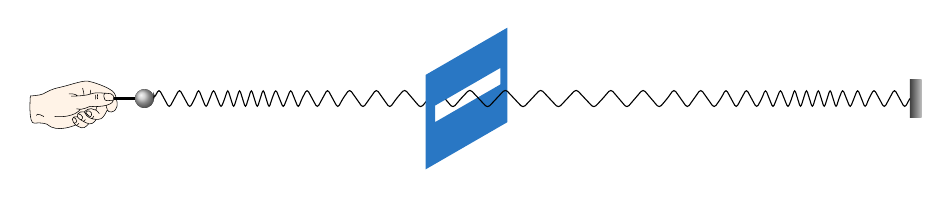
\begin{tikzpicture}[>=stealth,scale=0.6,samples=200]
  \begin{scope}
    \hand{xscale=-1}
    \draw[thick](1,0)--++(-0.85,0);
    \fill[ball color=lightgray] (0.8,0)circle(0.2);
    \draw[rounded corners=0.4mm]( 1.000, 0.0)--( 1.000, 0.0)--( 1.108, 0.2)--( 1.325,-0.2)--( 1.541, 0.2)--( 1.758,-0.2)--( 1.866, 0.0)--( 1.945, 0.2)--( 2.104,-0.2)--( 2.262, 0.2)--( 2.421,-0.2)--( 2.500, 0.0)--( 2.563, 0.2)--( 2.688,-0.2)--( 2.813, 0.2)--( 2.938,-0.2)--( 3.000, 0.0)--( 3.063, 0.2)--( 3.188,-0.2)--( 3.313, 0.2)--( 3.438,-0.2)--( 3.500, 0.0)--( 3.579, 0.2)--( 3.738,-0.2)--( 3.896, 0.2)--( 4.055,-0.2)--( 4.134, 0.0)--( 4.242, 0.2)--( 4.459,-0.2)--( 4.675, 0.2)--( 4.892,-0.2)--( 5.000, 0.0)--( 5.142, 0.2)--( 5.425,-0.2)--( 5.709, 0.2)--( 5.992,-0.2)--( 6.134, 0.0)--( 6.305, 0.2)--( 6.646,-0.2)--( 6.988, 0.2)--( 7.329,-0.2)--( 7.500, 0.0);

  \fill[left color=darkgray,right color=lightgray](17,-0.4)rectangle(17.25,0.4);
  \fill[azure5,even odd rule](6.75,-1.5)--++(30:2.0)--++(0,2)--++(210:2.0)--cycle(6.95,-0.5)--++(30:1.6)--++(0,0.35)--++(210:1.6)--cycle;
  \draw[rounded corners=0.4mm]( 7.500, 0.0)--( 7.688, 0.2)--( 8.063,-0.2)--( 8.438, 0.2)--( 8.813,-0.2)--( 9.000, 0.0)--( 9.187, 0.2)--( 9.562,-0.2)--( 9.937, 0.2)--(10.312,-0.2)--(10.500, 0.0)--(10.671, 0.2)--(11.012,-0.2)--(11.354, 0.2)--(11.695,-0.2)--(11.866, 0.0)--(12.008, 0.2)--(12.291,-0.2)--(12.575, 0.2)--(12.858,-0.2)--(13.000, 0.0)--(13.108, 0.2)--(13.325,-0.2)--(13.541, 0.2)--(13.758,-0.2)--(13.866, 0.0)--(13.945, 0.2)--(14.104,-0.2)--(14.262, 0.2)--(14.421,-0.2)--(14.500, 0.0)--(14.562, 0.2)--(14.687,-0.2)--(14.812, 0.2)--(14.937,-0.2)--(15.000, 0.0)--( 15.063, 0.2)--( 15.188,-0.2)--( 15.313, 0.2)--( 15.438,-0.2)--( 15.500, 0.0)--( 15.579, 0.2)--( 15.738,-0.2)--( 15.896, 0.2)--( 16.055,-0.2)--( 16.134, 0.0)--( 16.242, 0.2)--( 16.459,-0.2)--( 16.675, 0.2)--( 16.892,-0.2)--( 17.000, 0.0);
  \end{scope}
\end{tikzpicture}
\end{document}